\documentclass[11pt]{article}
%Gummi|065|=)
\title{\textbf{EV2.2.Arreglos y Parametros de los Amplificadores de clase A}}
\author{Cervantes Martinez Luis Osvaldo\\
		Sistemas Electronicos de Interfaz\\
		Martes, 1 de Octubre 2019}

\date{}
\usepackage{graphicx}
\begin{document}

\maketitle

\begin{figure}[htp]
\centering

\includegraphics[scale=0.5]{/home/osvaldo/Documentos/Interfaz/Tareas/EV2.2/UPZMG.png}
\label{}
\end{figure}
\pagebreak

\section{ Amplificadores de clase A}
Un amplificador clase A es aquel que representa a su salida una señal copia de la entrada, pero amplificada y sin distorsion.

 Los amplificadores emisores comunes son el tipo de amplificador mas comunmente usado, ya que pueden tener una ganancia de voltaje muy grande.
 
 Un amplificador de potencia funciona en clase A cuando la tension de polarizacion y la amplitud maxima de la señal de entrada poseen valores tales que hacen que la corriente de salida circule durante todo el periodo de la comunicacion de entrada.
\begin{figure}[htp]
\centering
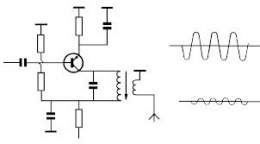
\includegraphics[scale=1.00]{/home/osvaldo/Documentos/Interfaz/Tareas/EV2.2/Amplificador.png}
\caption{Amplificador clase A}
\label{}
\end{figure}

\subsection{Ventajas y Desventajas}
Un solo dispositivo modulador. Sólo produce distorsión por la alinealidad del dispositivo. Esta clase es más teórica que práctica porque no se implementa en etapas reales pues dan poca potencia y bajo rendimiento. Son los que mejor suenan, los más cuestan y los menos prácticos. Despilfarran corriente y devuelven señales muy limpias. La clase A se refiere a una etapa de salida con una corriente de polarización mayor que la máxima corriente de salida que dan, de tal forma que los transistores de salida siempre están consumiendo corriente. La gran ventaja de la clase A es que es casi lineal, y en consecuencia la distorsión es menor.

La gran desventaja de la clase A es que es poco eficiente, es decir, que requiere un amplificador de clase A muy grande para dar 50 watts, y ese amplificador usa mucha corriente y se pone a muy alta temperatura.

Algunos amplificadores de high-end son clase A, pero la verdadera clase A sólo está en quizás un 10 porciiento del pequeño mercado de high-end y en ninguno del mercado de gama media.

Los amplificadores de clase A a menudo consisten en un transistor de salida conectado al positivo de la fuente de alimentación y un transistor de corriente constante conectado de la salida  al negativo de la fuente de alimentación.
La señal del transistor de salida modula tanto el voltaje como la corriente de salida. Cuando no  hay señal de entrada, la corriente de polarización constante fluye directamente del positivo de la fuente de alimentación al negativo, resultando que no hay corriente de salida, se gasta mucha corriente. Algunos amp de clase A más sofisticados tienen dos transistores de salida en configuracion push-pull



\end{document}
